\chapter{Sistemas y operaciones existentes}

El sistema que se propone en el presente OCD, tiene sus orígenes en el \acrfull{fua}.

Durante los últimos años de la década de 1980, el continuo crecimiento de la demanda de tráfico aéreo excedía la capacidad de los sistemas encargados de gestionarla, provocando retrasos significativos de las operaciones. Se reconoce por tanto la necesidad urgente de mejorar la gestión del espacio aéreo europeo, el concepto del FUA comienza a ser desarrollado por Eurocontrol en 1992. En este proceso participaron representantes civiles y militares de los Estados miembros. Fue finalmente introducido en marzo de 1996 en la mayoría de los países miembros de la \acrfull{ceac}.

No obstante, el concepto del FUA no se ha llegado a implementar completamente. El sistema que se ha desarrollado ha tenido una implantación desigual a lo largo del espacio aéreo europeo, alcanzando distintos niveles de desarrollo. Las conclusiones generales de aplicación del proceso no han sido satisfactorias, por lo que se ha comenzado a desarrollar una evolución de este concepto, el AFUA, que tratará de solventar los problemas a los que se ha enfrentado el FUA, y que será el objeto de este OCD.

\section{Misión del sistema existente}

Los objetivos y requisitos del espacio aéreo necesario para las operaciones varían en función de si los usuarios del espacio aéreo son civiles o militares. Mientras que la aviación civil busca encontrar aquellas trayectorias que le permitan volar las distintas rutas con la mayor eficiencia de costes posible, la aviación militar plantea sus operaciones de acuerdo con las rutas más eficientes para realizar sus misiones. 

Estas diferencias de planteamiento hacen imprescindible un análisis de la coordinación civil-militar necesaria para incrementar la eficiencia y capacidad del espacio aéreo. La eficiencia de las actuaciones de vuelo, así como volar las rutas más cortas, siempre han sido una de las prioridades principales del \acrfull{asm}.

El FUA se basa en el principio de que el espacio aéreo debe ser continuo y debe adaptarse a las necesidades de los usuarios (civiles y militares). Su puesta en marcha permite maximizar el uso del espacio aéreo mediante la coordinación civil-militar apropiada, logrando la separación requerida entre dichos vuelos y reduciendo la segregación del espacio aéreo.

Durante la fase implantación del FUA, estos son algunos de los objetivos que se fueron planteando:

\begin{itemize}
    \item \textbf{2005:} aplicación del FUA al espacio aéreo inferior, donde sea beneficioso.
    \item \textbf{2005:} expansión de la planificación del espacio aéreo con los estados vecinos para operaciones transfronterizas.
    \item \textbf{2006:} ampliación del FUA mediante la asignación dinámica de espacio aéreo para responder a cambios a corto plazo.
    \item \textbf{2006:} armonización de la manipulación del \acrfull{oat} / \acrfull{gat} en la mayor medida posible en toda Europa.
    \item \textbf{2008:} Introducción del \acrfull{cdm} del espacio aéreo europeo en consonancia con la estrategia de Cielo Único Europeo.
    \item \textbf{2015:} Avanzar hacia una función más integrada y que responda a la demanda para respaldar la responsabilidad colectiva de los Estados de la CEAC en la planificación y gestión del espacio aéreo europeo.
\end{itemize}

\section{Niveles de gestión}

El concepto de flexibilidad del espacio aéreo se desarrolla en tres niveles de gestión que corresponden a las tareas de coordinación civil-militar. Cada nivel de gestión está relacionado con el resto:

\begin{itemize}
    \item \textbf{Nivel 1. Estratégico.} Establecimiento de estructuras de espacio aéreo predeterminadas. Es la definición y revisión de alto nivel de la política nacional del espacio aéreo, teniendo en cuenta los requisitos de los usuarios del espacio aéreo nacional e internacional y de los proveedores ATS.
    
    Las tareas relacionadas incluyen el establecimiento de la organización del espacio aéreo, la planificación y la creación de estructuras permanentes y temporales del espacio aéreo y el acuerdo de prioridades y procedimientos de negociación.
    
    \item \textbf{Nivel 2. Pretáctico.} Asignación diaria del espacio aéreo en función de las necesidades de los usuarios. Es la realización de la gestión operativa en el marco de las estructuras y procedimientos definidos en el nivel 1.
    
    Las tareas pretácticas incluyen la asignación diaria del espacio aéreo y la comunicación de los datos de asignación del espacio aéreo a todas las partes involucradas.
    
    \item \textbf{Nivel 3. Táctico.} Utilización en tiempo real del espacio aéreo que permite una separación OAT/GAT segura. Consiste en la activación, desactivación o reasignación en tiempo real del espacio aéreo asignado en el Nivel 2 y en la resolución de problemas específicos del espacio aéreo y/o de situaciones individuales de tráfico entre el \acrfull{oat} y el \acrfull{gat}.
    
    Las tareas relacionadas incluyen el intercambio rápido de datos, con o sin apoyo del sistema, entre las unidades ATS civiles y militares pertinentes para permitir la realización segura y rápida de los vuelos de OAT y GAT.
\end{itemize}

\section{Estructura organizacional del FUA}\label{tit:fua_estructura}

El FUA está basado en adaptar la estructura del espacio aéreo para aquellas operaciones que necesitan hacer un uso temporal de este, como puede ser el caso de la actividad militar. Por consiguiente, es necesario definir un conjunto de estructuras flexibles, que permitan adaptarse a las necesidades de los operadores.

\begin{itemize}
    \item \textbf{Conditional Route (CDR):} son rutas que se planean y se usan bajo condiciones específicas, dependiendo del nivel de actividad esperado. Ver figura (\ref{fig:estructura_cdr}).
    \item \textbf{Temporary Reserved Area (TRA):} espacio aéreo reservado para un uso específico durante un determinado periodo de tiempo y cuyo uso será permitido solamente bajo el permiso del ATC. Ver figura (\ref{fig:estrutura_tsa_cba}).
    \item \textbf{Temporary Segregated Area (TSA):} espacio aéreo segregado y destinado a un solo usuario. La entrada y salida al mismo no estará permitido bajo ningún concepto. Ver figura (\ref{fig:estrutura_tsa_cba}).
    \item \textbf{Cross-Border Area (CBA):} son Temporary Reserved Area (TRA) y Temporary Segregated Area (TSA) establecidas sobre fronteras internacionales. Ver figura (\ref{fig:estrutura_tsa_cba}).
    \item \textbf{Prior co-ordination airspace (PCA):} es un espacio aéreo controlado donde se realizan actividades militares y al mismo tiempo aeronaves civiles pueden transitar bajo unas normas específicas. Ver figura (\ref{fig:estructura_rca}).
    \item \textbf{Reduced co-ordination airspace (RCA):} se trata de un espacio aéreo en el que apenas hay tráfico militar y en el que se permite que aeronaves civiles hagan uso del mismo. Ver figura (\ref{fig:estructura_rca}).
\end{itemize}

\begin{figure}[H]
    \centering
    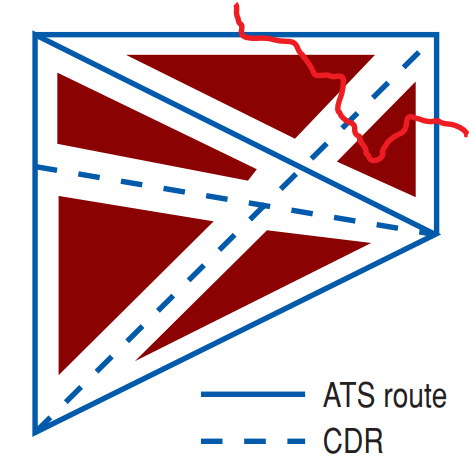
\includegraphics[width=0.25\linewidth]{figuras/estructura_cdr.png}
    \caption{Esquema de las rutas ATS convencionales y de las CDR.}
    \label{fig:estructura_cdr}
\end{figure}

\begin{figure}[H]
    \centering
    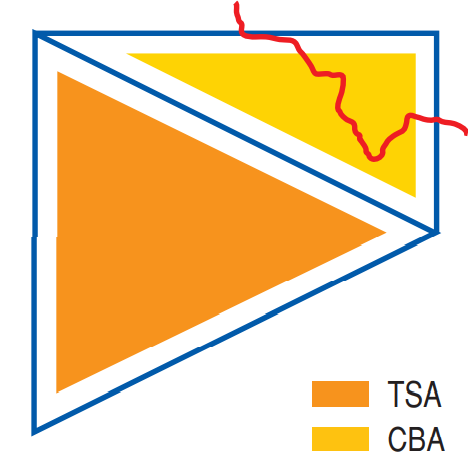
\includegraphics[width=0.25\linewidth]{figuras/estrutura_tsa_cba.png}
    \caption{Esquema de las áreas TRA, TSA y CBA.}
    \label{fig:estrutura_tsa_cba}
\end{figure}

\begin{figure}[H]
    \centering
    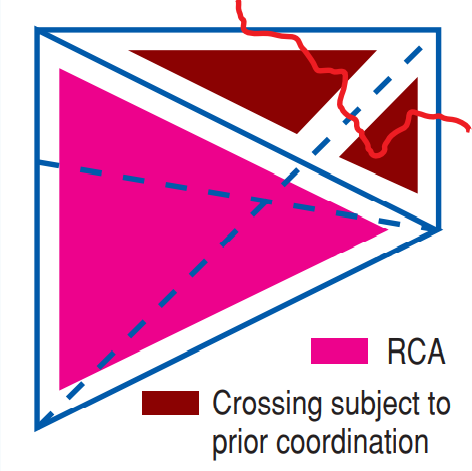
\includegraphics[width=0.25\linewidth]{figuras/estructura_rca.png}
    \caption{Esquema de las espacios aéreos PCA y RCA.}
    \label{fig:estructura_rca}
\end{figure}

\section{Entorno operativo del FUA}

Este sistema al operar en los Estados de la CEAC (Conferencia Europea de Aviación Civil) requiere que los Estados establezcan una coordinación civil y militar en tiempo real, que permita asignar estructuras flexibles de espacio aéreo diariamente. Para poner en marcha este sistema, se hará a través de los llamados “National Airspace Management Cells (ACMs)”, que se encargarán de asignar y promulgar la flexibilidad del espacio aéreo en base a la información que reciban tanto del entorno civil, como del militar.

Esta información a su vez la compartirán con el Network Manager (NM), cuyo cometido es difundir la disponibilidad diaria de las rutas ATS y la asignación diaria de los distintos espacios aéreos (restricciones, puntos intermedios obligatorios, etc). 

En la figura (\ref{fig:elementos_fua}) se puede observar el flujo de información descrito.

\begin{figure}[H]
    \centering
    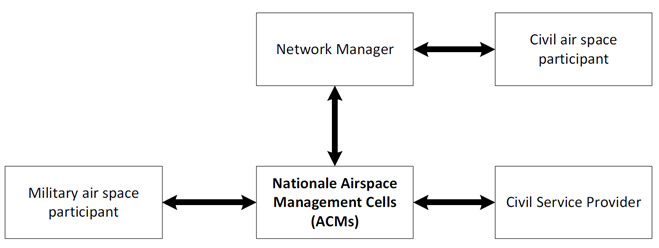
\includegraphics[width=1\linewidth]{figuras/elementos_fua.png}
    \caption{Elementos que constituyen el FUA.}
    \label{fig:elementos_fua}
\end{figure}

\section{Conclusiones y necesidad de un nuevo sistema}

Aunque como se ha comentado en la introducción de este apartado, la implementación del FUA ha sido desigual y no ha alcanzado todos los objetivos que se planteaban durante su periodo de definición, sí que se han observado algunas resultados positivos.

Entre estos aspectos positivos encontramos:

\begin{itemize}
    \item Se ha reducido la distancia, el tiempo y el combustible necesario para operar, mejorando la economía de los vuelos.
    \item Se ha incrementado la capacidad del sistema de control y se han reducido los retrasos.
    \item Se ha comprobado que funciona de manera más eficiente a la hora de separar operaciones civiles y militares.
    \item Ha permitido definir de manera más concreta las áreas de uso militar permitiendo que se adapten mejor a las necesidades de dichas operaciones.
\end{itemize}

Sin embargo, ya han aparecido nuevos proyectos que han hecho plantearse la necesidad de ir un paso más allá. En el horizonte aparece el AFUA, que realizará una revisión de lo conseguido hasta el momento, y buscará conseguir una coordinación aún mayor que permita aumentar aún más la capacidad y eficiencia del sistema de gestión del tránsito aéreo.

Durante la implantación del FUA, la integración del proceso de CDM mostró que aún existe un amplio margen de mejora. En particular, en la integración conjunta del \acrfull{asm}, \acrfull{atfcm} y el \acrfull{ats}, lo que permitirá disponer de más datos en tiempo real.

El propósito del sistema propuesto en este OCD, y que se comenzará a desarrollar a partir del apartado siguiente, será reemplazar las estructuras fijas por volúmenes de espacio aéreo con una configuración más dinámica, partiendo de la base de la cooperación civil–militar. Los avances que se consigan derivados de la implantación de este sistema darán como resultado la posibilidad de avanzar en otros sistemas como la \acrfull{dac}, el sistema Free Route y el \acrfull{swim}.

El conjunto integrado de todos estos sistemas permitirá dotar al espacio aéreo de una flexibilidad que será clave en un futuro en el que la demanda se haya incrementado notablemente.
